% P08-F04 bounded interaction renderer -- copied estimates only
%% source SHA256: 8c910290a3d09cbc9f03e7dcde77ae1598487533b0c68cfa1709a42e7d38621d
%% semantic SHA256: 7d136d1005cadbac7773e64dd39bb49d4ffc000a13fac4c4a3d1ee9c7742891a
\documentclass[border=0pt]{standalone}
\usepackage[T1]{fontenc}
\usepackage[utf8]{inputenc}
\usepackage{lmodern}
\usepackage{tikz}
\usepackage{pgfplots}
\pgfplotsset{compat=1.18}
\definecolor{PolA}{HTML}{0072B2}
\pgfplotsset{pt0/.style={only marks, mark=*, color=PolA, mark options={fill=PolA, draw=black}}}
\pgfplotsset{bar0/.style={PolA, line width=0.8pt, mark=|, mark options={color=PolA}}}
\definecolor{PolB}{HTML}{D55E00}
\pgfplotsset{pt1/.style={only marks, mark=square*, color=PolB, mark options={fill=PolB, draw=black}}}
\pgfplotsset{bar1/.style={PolB, line width=0.8pt, mark=|, mark options={color=PolB}}}
\pgfplotsset{domainpts/.style={only marks, mark=o, mark options={draw=gray, fill=none, scale=0.7}}}
\tikzset{intervalna/.style={font=\fontsize{8}{10}\selectfont, anchor=east}}
\begin{document}
\begin{minipage}{181.86mm}\centering
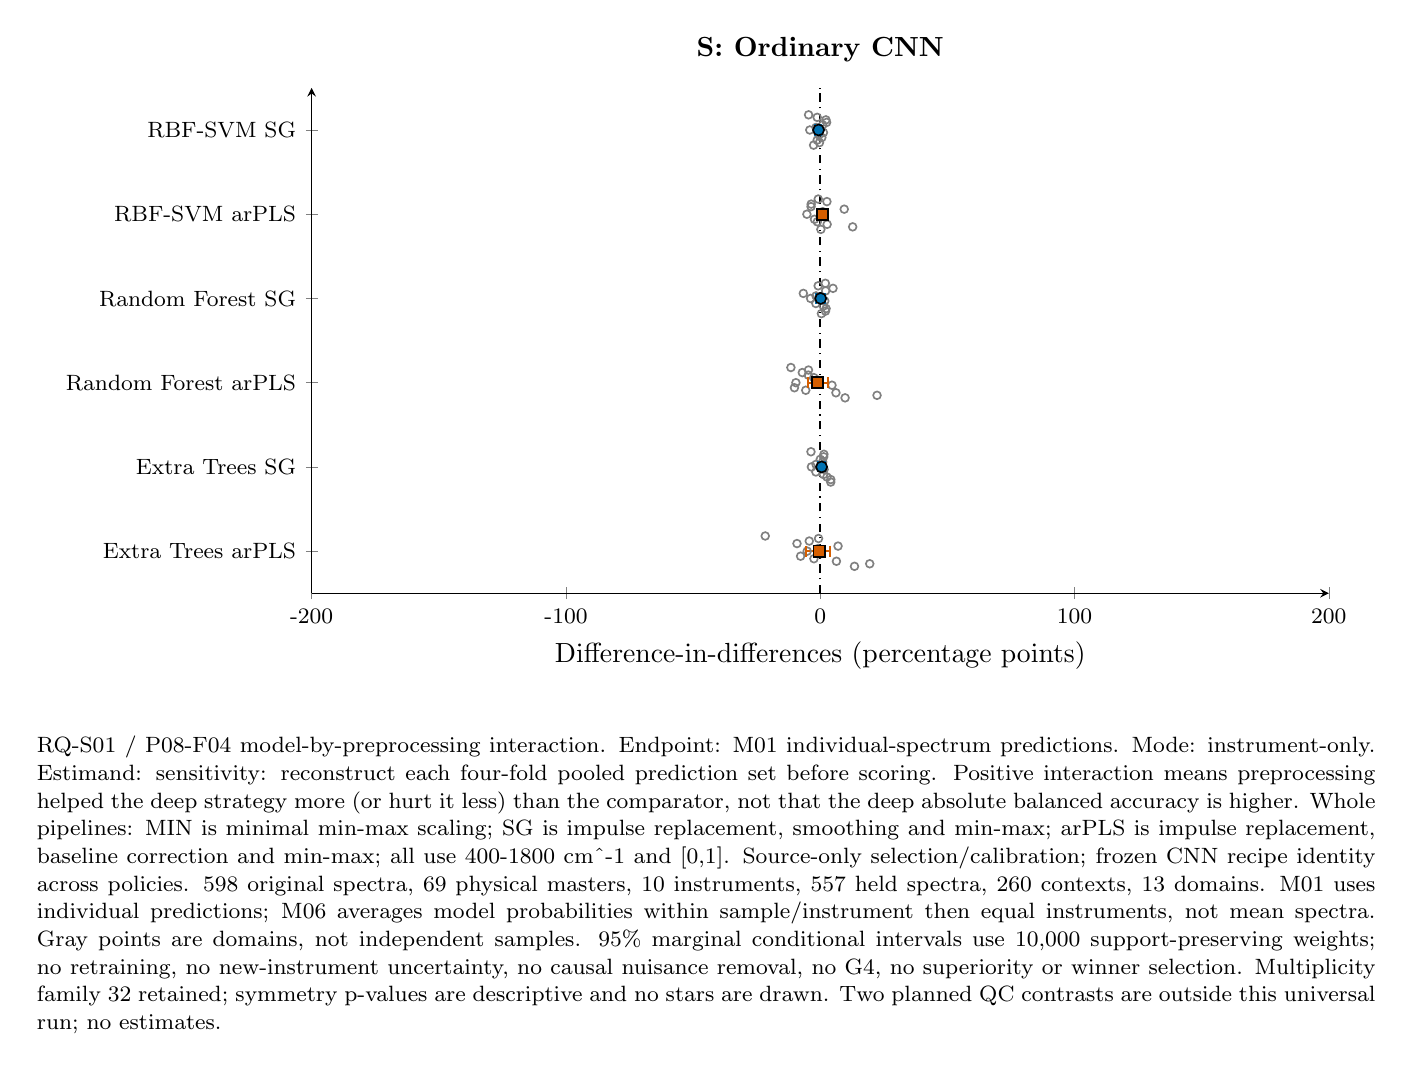
\begin{tikzpicture}
\begin{axis}[width=145mm, height=80mm, clip=false, xmin=-2, xmax=2, xtick={-2,-1,0,1,2}, xticklabels={-200,-100,0,100,200}, xlabel={Difference-in-differences (percentage points)}, ymin=-0.5, ymax=5.5, ytick={0,1,2,3,4,5}, yticklabels={{Extra Trees arPLS}, {Extra Trees SG}, {Random Forest arPLS}, {Random Forest SG}, {RBF-SVM arPLS}, {RBF-SVM SG}}, yticklabel style={font=\fontsize{8}{10}\selectfont}, tick label style={font=\fontsize{8}{10}\selectfont}, axis lines=left, title={S: Ordinary CNN}, title style={font=\bfseries\fontsize{10}{12}\selectfont}, every axis plot/.append style={line width=0.6pt}]
\draw[black, dash dot, line width=0.6pt] (axis cs:0,-0.5) -- (axis cs:0,5.5);
\addplot[domainpts] coordinates {(-0.026269841269841269,4.8200000000000003) (-0.0031534391534391512,4.8499999999999996) (-0.012121212121212123,4.8799999999999999) (0.0060606060606060606,4.9100000000000001) (-0.0051282051282051291,4.9400000000000004) (0.012301075268817204,4.9699999999999998) (-0.041203703703703701,5) (-0.01666666666666667,5.0300000000000002) (0.0095238095238095229,5.0599999999999996) (0.024915824915824919,5.0899999999999999) (0.022121212121212125,5.1200000000000001) (-0.012142857142857141,5.1500000000000004) (-0.045977011494252866,5.1799999999999997)};
\addplot[bar0] coordinates {(-0.019380625982212889,5) (0.0037819242132496531,5)};
\addplot[pt0] coordinates {(-0.006749262214608324,5)};
\addplot[domainpts] coordinates {(0.0023015873015872997,3.8199999999999998) (0.12738624338624341,3.8500000000000001) (0.02690909090909091,3.8799999999999999) (-0.011666666666666667,3.9100000000000001) (-0.022843822843822848,3.9399999999999999) (-0.00013978494623655691,3.9700000000000002) (-0.052645502645502641,4) (0.0095238095238095229,4.0300000000000002) (0.094179894179894169,4.0599999999999996) (-0.036363636363636376,4.0899999999999999) (-0.035757575757575766,4.1200000000000001) (0.026111111111111106,4.1500000000000004) (-0.0080459770114942528,4.1799999999999997)};
\addplot[bar1] coordinates {(-0.010971173711522661,4) (0.02513579770826542,4)};
\addplot[pt1] coordinates {(0.0091499053982154847,4)};
\addplot[domainpts] coordinates {(0.0045238095238095246,2.8199999999999998) (0.020529100529100529,2.8500000000000001) (0.022787878787878788,2.8799999999999999) (0.012121212121212121,2.9100000000000001) (-0.01724941724941725,2.9399999999999999) (0.017634408602150538,2.9700000000000002) (-0.037962962962962962,3) (-0.01666666666666667,3.0299999999999998) (-0.066666666666666666,3.0600000000000001) (0.02087542087542088,3.0899999999999999) (0.049999999999999996,3.1200000000000001) (-0.008333333333333335,3.1499999999999999) (0.019923371647509583,3.1800000000000002)};
\addplot[bar0] coordinates {(-0.016322178118243956,3) (0.018192648082912592,3)};
\addplot[pt0] coordinates {(0.0016550888621565444,3)};
\addplot[domainpts] coordinates {(0.097539682539682537,1.8200000000000001) (0.22315343915343916,1.8500000000000001) (0.061575757575757575,1.8799999999999999) (-0.057121212121212114,1.9099999999999999) (-0.10163170163170163,1.9399999999999999) (0.046037634408602146,1.97) (-0.095899470899470901,2) (-0.0095238095238095229,2.0299999999999998) (-0.025396825396825397,2.0600000000000001) (-0.047138047138047146,2.0899999999999999) (-0.070606060606060603,2.1200000000000001) (-0.046428571428571423,2.1499999999999999) (-0.11551724137931034,2.1800000000000002)};
\addplot[bar1] coordinates {(-0.049501601551465997,2) (0.031332015534693246,2)};
\addplot[pt1] coordinates {(-0.010842802034425204,2)};
\addplot[domainpts] coordinates {(0.041190476190476187,0.82000000000000006) (0.041248677248677243,0.84999999999999998) (0.026181818181818185,0.88) (0.012727272727272729,0.91000000000000003) (-0.01724941724941725,0.93999999999999995) (0.014967741935483872,0.96999999999999997) (-0.034854497354497346,1) (-0.01666666666666667,1.03) (0.0095238095238095229,1.0600000000000001) (2.7755575615628915e-18,1.0900000000000001) (0.013333333333333331,1.1200000000000001) (0.014285714285714285,1.1499999999999999) (-0.036590038314176246,1.1799999999999999)};
\addplot[bar0] coordinates {(-0.0081245213124192979,1) (0.017544421127118362,1)};
\addplot[pt0] coordinates {(0.0052383249109098345,1)};
\addplot[domainpts] coordinates {(0.13452380952380952,-0.17999999999999999) (0.1944973544973545,-0.14999999999999999) (0.063515151515151497,-0.12) (-0.025000000000000001,-0.089999999999999997) (-0.077389277389277394,-0.059999999999999998) (0.0019462365591397877,-0.029999999999999999) (-0.051455026455026455,0) (-0.0095238095238095229,0.029999999999999999) (0.069841269841269843,0.059999999999999998) (-0.091582491582491571,0.089999999999999997) (-0.043333333333333335,0.12) (-0.0068253968253968247,0.14999999999999999) (-0.21647509578544061,0.17999999999999999)};
\addplot[bar1] coordinates {(-0.056896980610885016,0) (0.038585329386907653,0)};
\addplot[pt1] coordinates {(-0.0044046622275423514,0)};
\end{axis}
\node[anchor=north, align=justify, text width=170mm, font=\fontsize{8}{10}\selectfont] at ([yshift=-6mm]current bounding box.south) {RQ-S01 / P08-F04 model-by-preprocessing interaction. Endpoint: M01 individual-spectrum predictions. Mode: instrument-only. Estimand: sensitivity: reconstruct each four-fold pooled prediction set before scoring. Positive interaction means preprocessing helped the deep strategy more (or hurt it less) than the comparator, not that the deep absolute balanced accuracy is higher. Whole pipelines: MIN is minimal min-max scaling; SG is impulse replacement, smoothing and min-max; arPLS is impulse replacement, baseline correction and min-max; all use 400-1800 cm\textasciicircum{}-1 and [0,1]. Source-only selection/calibration; frozen CNN recipe identity across policies. 598 original spectra, 69 physical masters, 10 instruments, 557 held spectra, 260 contexts, 13 domains. M01 uses individual predictions; M06 averages model probabilities within sample/instrument then equal instruments, not mean spectra. Gray points are domains, not independent samples. 95\% marginal conditional intervals use 10,000 support-preserving weights; no retraining, no new-instrument uncertainty, no causal nuisance removal, no G4, no superiority or winner selection. Multiplicity family 32 retained; symmetry p-values are descriptive and no stars are drawn. Two planned QC contrasts are outside this universal run; no estimates.};
\end{tikzpicture}
\end{minipage}
\end{document}
